% Source locale antérieure au PDF final ; voir report/README.md.
% Compiler depuis report/ ; le PDF fourni est conservé sans modification.
% Encodage : UTF-8. Compilation : pdfLaTeX, deux passages.
% Dans Overleaf, conserver rapportECL.cls et les ressources de votre modèle.
% En leur absence, une mise en page article permet de relire le même texte.
% Les images sont chargées depuis ../figures/ (minuscules), comme dans Overleaf.
% La couverture et le sommaire occupent chacun une page non numérotée.
% Le corps du rapport commence ensuite à la page 1, en pagination continue.
%
% Sources locales utilisées pour la rédaction et les chiffres :
% docs/assignment/BE_CS1_instructions.ipynb
% outputs/tables/eda_metrics.json et parsing_audit.json
% src/parser.py, features.py, train_eval.py, optimize_models.py, postprocess.py
% src/nested_validation.py et sinkhorn_positional_ensemble.py
% outputs/tables/benchmark_results.csv, optimization_ablation.csv
% outputs/tables/dl_hybrid_audit.md (limites des premiers prétraitements)
% Chronologie des scores publics : précisions et texte fournis par le groupe.
% Le score OOF optimisé est présenté comme un résultat de sélection.
% Les essais positionnels et de rééquilibrage ne constituent pas une ablation
% indépendante : la branche historique contient aussi des choix par ligne.

\newif\ifclasseECL
\IfFileExists{rapportECL.cls}{\classeECLtrue}{\classeECLfalse}
\ifclasseECL
  \documentclass{rapportECL}
\else
  \documentclass[11pt,a4paper]{article}
  \usepackage[margin=2.3cm]{geometry}
\fi
\usepackage[utf8]{inputenc}
\usepackage[T1]{fontenc}
\usepackage{lmodern}
\usepackage[french]{babel}
\usepackage{graphicx}
\usepackage{hyperref}
\hypersetup{hidelinks,hypertexnames=false}
\setlength{\parindent}{0pt}
\setlength{\parskip}{0.35em}
\setlength{\tabcolsep}{6pt}
\renewcommand{\arraystretch}{1.12}
\emergencystretch=1.5em
\raggedbottom

% Éviter que les illustrations bloquent le texte et laissent une page vide.
\setcounter{topnumber}{3}
\setcounter{bottomnumber}{2}
\setcounter{totalnumber}{5}
\renewcommand{\topfraction}{0.90}
\renewcommand{\bottomfraction}{0.85}
\renewcommand{\textfraction}{0.10}
\renewcommand{\floatpagefraction}{0.75}
\setlength{\floatsep}{8pt plus 2pt minus 2pt}
\setlength{\textfloatsep}{10pt plus 2pt minus 2pt}
\setlength{\intextsep}{8pt plus 2pt minus 2pt}
\setlength{\abovecaptionskip}{5pt}
\setlength{\belowcaptionskip}{2pt}

% Déposer les cinq graphiques et la capture de Copilote dans ../figures/.
% Nom prévu pour la capture : assets/copilote_usine_cliquable.png.
% La casse du dossier et des noms de fichiers doit correspondre exactement.
\newcommand{\figurerepere}[3]{%
  \begin{figure}[!htbp]
    \centering
    \includegraphics[width=0.90\linewidth,height=0.22\textheight,keepaspectratio]{#1}
    \caption{#2}\label{#3}
  \end{figure}
}

\title{BE -- Identification des utilisateurs de Copilote}
\begin{document}
\pagenumbering{gobble}

\ifclasseECL
  \titre{Identification des utilisateurs de Copilote}
  \UE{MOD 7.2 : Introduction aux sciences des données}
  \sujet{Rendu BE 1}
  \enseignant{Antoine \textsc{Becquet}\break}
  \eleves{Abderrazak \textsc{Khalil}\break
          Salma \textsc{Ihssane}\break
          Anas \textsc{Meniari}\break}
  \fairemarges
  \fairepagedegarde
\else
  \begin{titlepage}
    \centering
    {\large École Centrale de Lyon\par}
    \vspace{1.5cm}
    {\large MOD 7.2 -- Introduction aux sciences des données\par}
    \vfill
    {\LARGE\bfseries Identification des utilisateurs\\[0.3em]de Copilote\par}
    \vspace{0.8cm}
    {\large Rendu BE 1\par}
    \vfill
    Abderrazak \textsc{Khalil}\\
    Salma \textsc{Ihssane}\\
    Anas \textsc{Meniari}\par
    \vspace{1cm}
    Enseignant : Antoine \textsc{Becquet}\par
    \vspace{1cm}
    Novembre 2026
  \end{titlepage}
\fi

% Sommaire seul sur sa page ; aucun numéro avant le début du rapport.
\clearpage
\thispagestyle{empty}
\begingroup
  \small
  \setlength{\parskip}{0pt}
  \setcounter{tocdepth}{2}
  \tableofcontents
\endgroup
\clearpage
\pagenumbering{arabic}

% =====================================================================
% Problème, audit de forme et cible
% =====================================================================
\section{Comprendre les traces avant de construire un modèle}

Peut-on reconnaître une personne à sa manière d'utiliser un logiciel ? C'est la question que nous avons étudiée à partir des traces de l'ERP Copilote, développé par Infologic. Chaque session rassemble un navigateur, des actions et des repères temporels ; nous devons lui attribuer l'un des \textbf{247 utilisateurs} présents dans l'apprentissage.

Pour mieux comprendre à quoi correspondaient ces traces, nous avons aussi consulté la présentation de Copilote proposée par Infologic, notamment son \og usine cliquable \fg{} (figure~\ref{fig:copilote}). Elle situe les usages dans leur contexte métier : réceptions et stocks, fabrication, préparation, expéditions et administratif. Cette vue nous a aidés à rapprocher les actions et les écrans des parcours de travail possibles dans l'ERP.

\begin{figure}[!htbp]
  \centering
  % Déposer la capture jointe sous ce nom dans Overleaf.
  \IfFileExists{assets/copilote_usine_cliquable.png}{%
    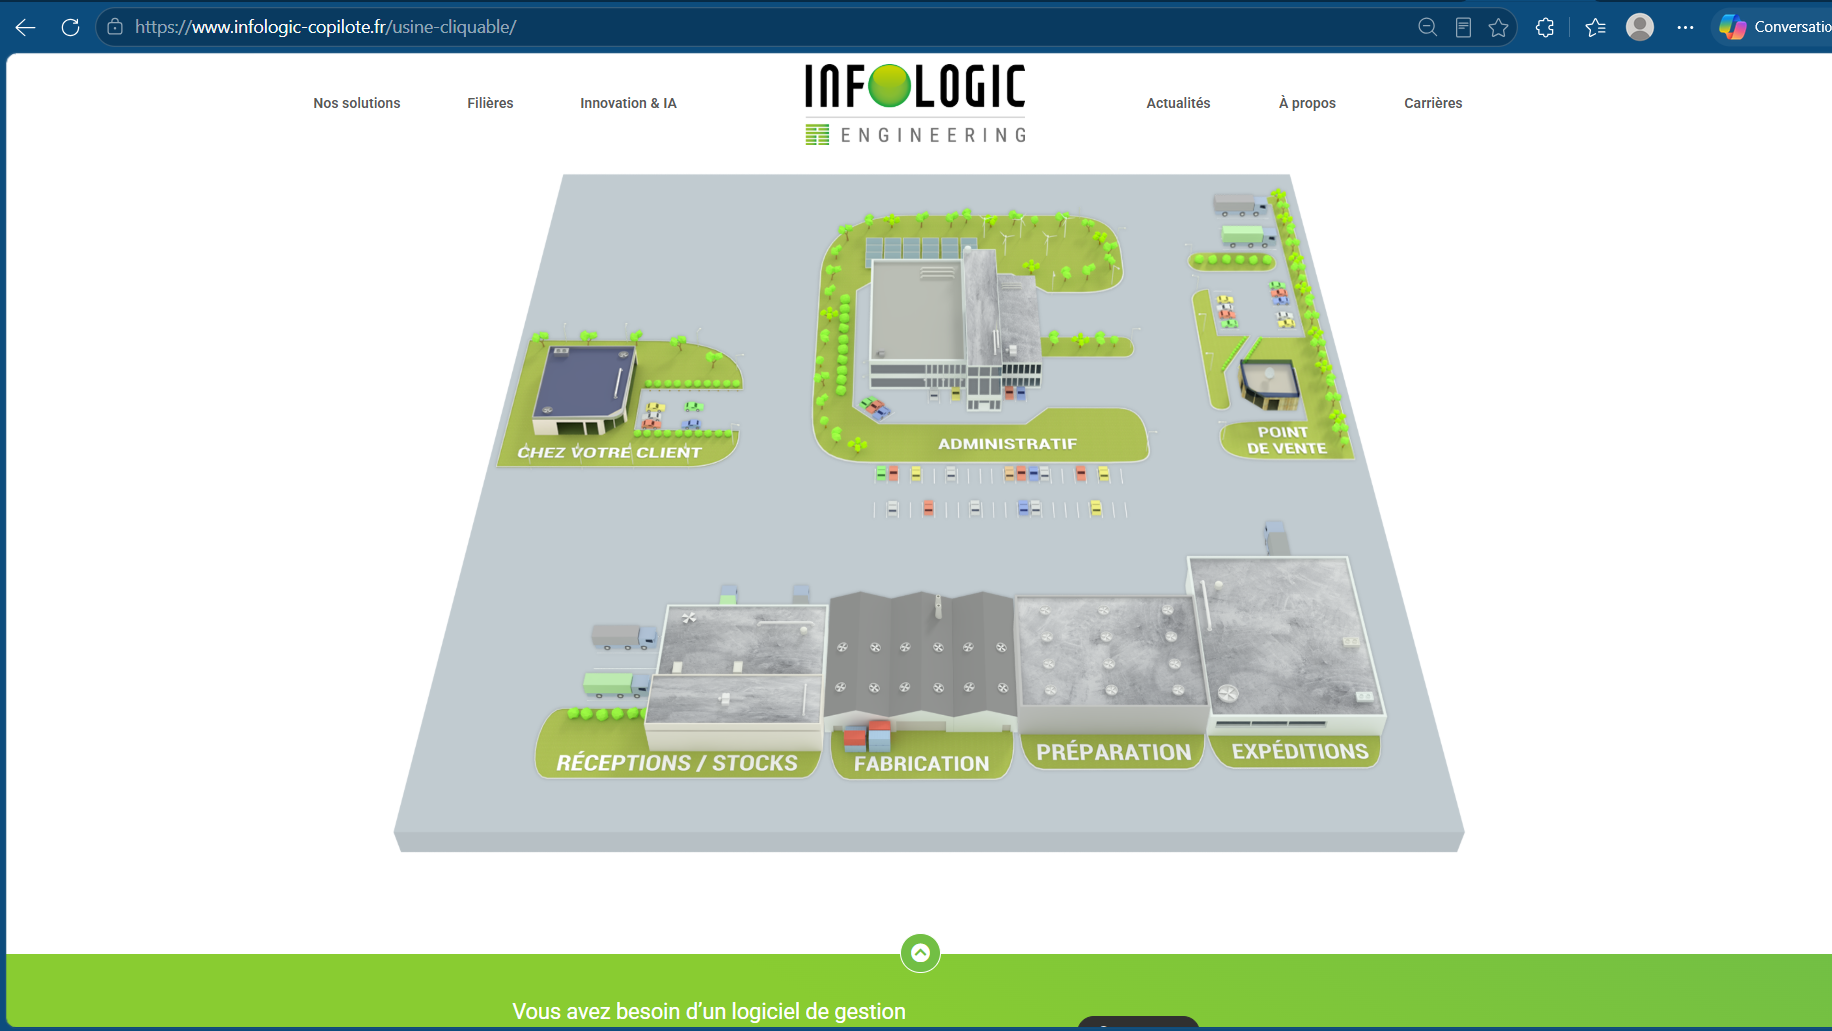
\includegraphics[width=0.90\linewidth,height=0.22\textheight,keepaspectratio]{assets/copilote_usine_cliquable.png}%
  }{%
    \fbox{\parbox[c][0.22\textheight][c]{0.85\linewidth}{\centering
      Capture de l'usine cliquable à ajouter :\\[0.5em]
      \nolinkurl{assets/copilote_usine_cliquable.png}}}%
  }
  \caption[Vue de l'usine cliquable d'Infologic]{Vue de l'\og usine cliquable \fg{}, consultée pour situer les activités couvertes par Copilote. Source : \href{https://www.infologic-copilote.fr/usine-cliquable/}{Infologic}.}
  \label{fig:copilote}
\end{figure}

La préparation a pris une grande place dans notre travail. Avant de comparer les modèles, il nous fallait comprendre ce que contenaient les lignes et ce que nous pouvions réellement en tirer. Nous avons organisé cette exploration en cinq analyses, avec l'idée de faire suivre chaque observation d'une décision pour la suite. Ce lien entre comprendre les données et choisir une méthode a été au centre de notre apprentissage.

\subsection{Audit de forme et de volume}

Nous avons commencé par lire les fichiers bruts. Une ligne correspond à une session, mais les lignes n'ont pas toutes la même longueur. Dans le train, les deux premiers champs donnent l'utilisateur et le navigateur ; dans le test, seul le navigateur précède les événements. Une lecture ligne par ligne nous permet de garder cette structure sans créer artificiellement des milliers de colonnes vides pour les sessions courtes.

\begin{table}[!htbp]
\centering\small
\begin{tabular}{lrr}
\hline
 & Apprentissage & Test \\
\hline
Nombre de sessions & 3\,279 & 324 \\
Nombre médian d'actions & 340 & 365 \\
Nombre moyen d'actions & 692,4 & 662,3 \\
Nombre maximal d'actions & 11\,977 & 6\,203 \\
\hline
\end{tabular}
\caption{Volume des données, en comptant les actions séparément des horloges.}
\end{table}

La moyenne dépasse largement la médiane : quelques sessions très longues tirent les valeurs vers le haut. Nous avons aussi repéré trois sessions d'apprentissage avec moins de cinq actions, dont une sans action. Cela nous a conduits à privilégier des fréquences relatives et des transformations logarithmiques plutôt que des comptes bruts seuls. Une session longue ne doit pas peser davantage uniquement parce qu'elle contient plus d'événements.

\figurerepere{../figures/fig1_sequence_lengths.png}{Longueurs des sessions : une forte hétérogénéité dans les deux ensembles.}{fig:longueurs}

\subsection{Analyse de la cible}

Les utilisateurs ont entre \textbf{4 et 75 sessions}, avec une médiane de 12 ; 33 personnes n'en ont pas plus de cinq. Ce déséquilibre pose deux questions : comment apprendre avec peu d'exemples et comment évaluer sans privilégier les utilisateurs fréquents ? Nous avons retenu le Macro-F1 et une validation stratifiée à quatre plis. Le minimum de quatre sessions nous donne ici le nombre maximal de plis permettant de représenter chaque utilisateur dans chaque validation externe.

\figurerepere{../figures/fig2_target_imbalance.png}{Répartition des sessions par utilisateur et concentration des effectifs.}{fig:cible}

% =====================================================================
% Alignement, sparsité et structure des tokens
% =====================================================================
\subsection{Alignement entre apprentissage et test}

Nous avons ensuite comparé les deux ensembles pour vérifier si les habitudes apprises semblaient transférables au test. Les longueurs de sessions ont des ordres de grandeur proches, malgré des extrêmes différents. La répartition des navigateurs est également voisine : Firefox représente 44,7\,\% du train et 45,4\,\% du test, Chrome 40,8\,\% et 41,0\,\%. Nous n'observons donc pas de décalage majeur sur ces caractéristiques. Cette comparaison reste partielle : elle ne suffit pas à exclure un \emph{covariate shift} sur l'ensemble des comportements.

Un autre constat nous a particulièrement servi : \textbf{les 247 utilisateurs conservent chacun le même navigateur dans le train}. Le navigateur devient alors une information de contexte utile pour réduire les identités possibles. Nous avons encodé cette variable par indicatrices, puis utilisé cette fidélité pour filtrer les sorties des modèles. Elle reste une régularité du jeu observé ; un changement de navigateur pourrait la mettre en défaut.

\figurerepere{../figures/fig3_browser_analysis.png}{Comparaison train/test et fidélité des utilisateurs à leur navigateur.}{fig:navigateurs}

\subsection{Sparsité et décomposition des actions}

Nous avons ensuite regardé ce que signifierait encoder directement chaque événement. Le train contient \textbf{7\,086 tokens distincts}, dont 28\,\% apparaissent une seule fois et 56,5\,\% au plus cinq fois. Dans le vocabulaire distinct du test, 206 tokens complets sont nouveaux, soit 7,3\,\%. Un encodage limité aux événements entiers laisserait donc beaucoup de motifs rares et quelques événements sans représentation connue.

Heureusement, les actions suivent une structure exploitable :
\begin{center}
\verb|Action(Controleur)<Configuration>$Domaine$1|
\end{center}
Les composants après l'action sont optionnels. Ils nous permettent de distinguer le geste, l'écran, sa configuration et le domaine concerné. Nous avons donc conservé à la fois le token complet et ses composants : deux événements différents peuvent ainsi partager une partie de leur information.

\begin{table}[!htbp]
\centering\small
\begin{tabular}{lrr}
\hline
Niveau & Vocabulaire du train & Éléments nouveaux du test \\
\hline
Action de base & 35 & 0 \\
Contrôleur & 415 & 8 \\
Configuration & 219 & 2 \\
Domaine & 76 & 0 \\
\hline
\end{tabular}
\caption{La décomposition réduit la difficulté liée aux événements inconnus.}
\end{table}

La lecture a aussi révélé des exceptions concrètes : un marqueur \texttt{t5} collé à une action par une virgule manquante, et des parenthèses imbriquées dans des traces Java. Nous avons prévu leur traitement dans le parseur pour éviter de créer de fausses catégories. Ce travail de détail nous a montré qu'un événement mal découpé peut modifier aussi bien le vocabulaire que les calculs temporels.

\figurerepere{../figures/fig4_sparsity_and_parsing.png}{Rareté des tokens bruts et intérêt de leur décomposition.}{fig:sparsite}

% =====================================================================
% Dynamique et deux représentations
% =====================================================================
\subsection{Dynamique séquentielle et temporelle}

La dernière analyse porte sur la manière dont les actions s'enchaînent. L'exécution d'un bouton représente 22,49\,\% des actions, la saisie 11,70\,\% et la sélection d'un écran 9,11\,\%. Ces gestes sont courants : leur présence seule ne suffit pas à reconnaître quelqu'un. En revanche, leurs proportions, leurs répétitions et leurs enchaînements peuvent décrire des habitudes. Nous observons notamment \textbf{18,08\,\% de répétitions immédiates d'une même action de base} parmi les transitions.

Les marqueurs \texttt{tX} ajoutent une dimension de rythme. La durée médiane estimée à partir du dernier marqueur vaut 395 secondes. Nous avons construit des statistiques d'activité par fenêtres de cinq secondes, mais ces repères ne donnent pas l'heure exacte de chaque clic. Nous avons aussi rencontré des marqueurs successifs de même valeur : ces intervalles nuls doivent être traités sans division par zéro. Les débits calculés décrivent donc une activité agrégée, à interpréter en tenant compte de la précision de l'enregistrement.

Nous avons retenu de cette étape trois compléments au contenu : les courts motifs d'actions, les longueurs de séries répétées et les statistiques temporelles. Il nous semblait utile de conserver ces informations plutôt que de réduire une session à la liste des écrans visités.

\figurerepere{../figures/fig5_temporal_and_actions.png}{Durées des sessions et principales actions observées.}{fig:dynamique}

\section{Transformer les sessions en variables d'apprentissage}
\subsection{Une première représentation par les actions et leurs motifs}

Notre première approche consiste à traiter une session comme un document et ses événements comme des mots. Un \emph{Bag of Words} fournit une base, mais ses comptes bruts sont sensibles aux répétitions et à la longueur des sessions. Nous avons donc utilisé un \textbf{TF-IDF à fréquence sous-linéaire}, avec normalisation L2 de chaque bloc : les répétitions sont atténuées et les motifs présents dans presque toutes les sessions reçoivent moins de poids.

Nous avons appliqué cette représentation aux tokens complets et aux composants extraits. Les unigrammes décrivent le contenu ; les bigrammes et, pour les actions, les trigrammes conservent de courts enchaînements. Des indicatrices de début et de fin complètent cette vue. Pour limiter la dimension, nous avons fixé des seuils de présence dans plusieurs sessions et des plafonds de vocabulaire. Le découpage préalable préserve les noms d'actions contenant des espaces : une action reste bien une unité du vocabulaire.

\subsection{Une seconde représentation par le comportement global}

En parallèle, nous avons construit une table de \textbf{246 descripteurs comportementaux} dans le cache initial : volume et durée, diversité des écrans, fréquences relatives des actions et domaines, entropies, répétitions consécutives et rythme. Nous avons aussi représenté les transitions entre les dix actions les plus fréquentes par une matrice de 100 valeurs. Cette seconde approche résume la façon d'utiliser le logiciel, avec des variables plus faciles à interpréter individuellement. Les deux représentations décrivent ainsi les mêmes sessions à des niveaux différents.

% =====================================================================
% Hybride, validation et modèles classiques
% =====================================================================
\subsection{Combiner les deux représentations sans écraser un signal}

L'hybride nous paraissait naturel : associer les motifs précis du TF-IDF aux statistiques globales. Mais notre première concaténation donnait de moins bons résultats que le TF-IDF seul. Ce point a été instructif : ajouter des variables utiles séparément ne garantit pas qu'elles fonctionneront bien ensemble. Leur échelle et leur poids relatif comptent aussi.

Nous avons standardisé les descripteurs comportementaux, normalisé leur vecteur par session, puis réduit leur poids avant la concaténation avec le TF-IDF. La version retenue utilise un coefficient de 0,25 pour ce bloc, issu de nos premiers réglages. Les statistiques peuvent ainsi compléter les motifs sans prendre le dessus par leur seule amplitude. Ce changement nous a davantage appris qu'un simple ajustement d'hyperparamètre : il fallait d'abord rendre les informations comparables pour que leur association ait un sens.

\section{Faire progresser la solution par étapes}
\subsection{Croiser trois représentations et cinq familles de modèles}

Notre idée de départ était de reconnaître à la fois les tâches réalisées et la manière de les enchaîner. Nous avons donc confronté \textbf{cinq familles de modèles} aux trois représentations construites : régression logistique, SVM linéaire, MLP, arbre de décision et XGBoost. Ces quinze combinaisons devaient nous aider à comprendre ce que chaque représentation rendait accessible à l'apprentissage.

Les modèles linéaires nous donnaient une référence sur le TF-IDF creux ; les arbres et le MLP permettaient d'explorer d'autres relations entre les variables. Pour l'arbre, XGBoost et le MLP, le bloc lexical était réduit par SVD dans chaque pli. Nous pouvions ainsi comparer plusieurs façons d'exploiter les mêmes sessions, plutôt que choisir un algorithme avant d'avoir observé ses résultats.

\begin{table}[!htbp]
\centering\small
\begin{tabular}{lrrr}
\hline
Modèle & TF-IDF & Comportement & Hybride initial \\
\hline
Régression logistique & 92,36 & 46,93 & 86,76 \\
SVM linéaire & \textbf{96,20} & 65,28 & 87,54 \\
MLP & 87,05 & 77,67 & 85,54 \\
Arbre de décision & 19,28 & 65,61 & 62,15 \\
XGBoost & 71,70 & 83,01 & \textbf{85,62} \\
\hline
\end{tabular}
\caption{Macro-F1 (\%) après masque navigateur dans le benchmark exploratoire des cinq modèles.}
\end{table}

Cette comparaison nous a orientés : le SVM exploitait très bien les motifs lexicaux, tandis que XGBoost tirait davantage parti des statistiques et de l'hybride. Elle a aussi révélé le problème d'échelle décrit précédemment : notre hybride initial donnait seulement 87,54\,\% de Macro-F1 avec le SVM, contre 96,20\,\% pour le TF-IDF seul. Après normalisation des blocs et réglage, le SVM hybride atteignait 96,38\,\%. L'information ajoutée pouvait donc devenir utile, à condition de lui donner une place adaptée.

\subsection{Construire un vote plutôt que retenir un seul gagnant}

Nous avons d'abord réuni les cinq familles dans un \textbf{vote souple pondéré}, en retenant pour chacune sa représentation la plus convaincante. Ce vote combine les scores attribués aux utilisateurs, et pas seulement les étiquettes finales. Les marges du SVM sont transformées par softmax ; leur mise à l'échelle contrôle leur influence dans l'ensemble, sans en faire une mesure exacte de confiance.

Le navigateur nous a permis de traduire un autre constat de l'EDA en règle de décision : annuler les scores des identités incompatibles avec celui de la session, puis renormaliser. Dans le benchmark, ce filtre fait passer le SVM lexical de 94,17\,\% à 96,20\,\% de Macro-F1. Son intérêt dépend de la fidélité au navigateur observée dans les données.

\textbf{Notre première soumission Kaggle a obtenu un score public de 97,4\,\%.} Ce premier palier venait du travail sur les représentations, leur normalisation et la combinaison de modèles classiques. Pour produire le fichier, nous moyennons les probabilités test des quatre plis, appliquons le vote et conservons les 324 sessions au format \texttt{RowId,prediction}.

\subsection{Mieux distinguer choisir une méthode et l'évaluer}

Dès les premiers essais, nous avons suivi l'\textbf{accuracy} et le \textbf{Macro-F1}, ce dernier donnant autant de poids à chaque utilisateur. La validation stratifiée à quatre plis, avec mélange et graine 42, fournit des prédictions hors pli, ou OOF : chaque session est prédite par un modèle qui ne l'a pas utilisée pour apprendre.

Ces prédictions nous ont servi à régler les modèles et les poids du vote. Nous avons alors mieux compris une difficulté : un score utilisé pour sélectionner des poids n'est plus une évaluation indépendante de ces poids. Nous avons donc introduit une \textbf{validation imbriquée}, avec des plis internes pour choisir les réglages et un pli externe pour évaluer le choix retenu.

Nous avons aussi identifié des transformations initialement ajustées sur tout le train avant le découpage. Le protocole a ensuite été revu pour les réapprendre dans chaque sous-ensemble d'entraînement. Les premiers scores restent exploratoires ; cette correction nous a appris à vérifier la séparation des données dès la construction des variables, pas uniquement au moment d'entraîner le classifieur.

\subsection{Comprendre ce que les autres modèles apportent au meilleur}

Les réglages de régularisation et de sélection de variables ont amélioré les candidats. Nous avons également ajouté \textbf{Ridge}, particulièrement efficace sur l'hybride normalisé. Un vote ultérieur réunissait alors deux SVM, Ridge, la régression logistique et le MLP. Ridge obtenait 97,04\,\% de Macro-F1 OOF et le vote optimisé 97,94\,\%, avec un poids dominant pour Ridge. Ce dernier score servait à sélectionner la combinaison ; nous le distinguons donc d'une mesure indépendante de généralisation.

Une simplification autour de Ridge et du SVM a pourtant ramené le score public à \textbf{97,2\,\%}, contre 97,4\,\% pour notre première soumission. Ce recul a remis en question l'idée de ne garder que les meilleurs modèles individuels. Il suggérait que d'autres candidats pouvaient encore aider sur certaines ambiguïtés. Les poids et la composition ayant changé ensemble, cette comparaison ne prouve pas l'apport isolé de chacun ; elle nous a surtout conduits à examiner leurs désaccords avant de les écarter.

\subsection{Revenir aux sessions pour chercher des indices plus précis}

Pour poursuivre, nous sommes revenus à la représentation des traces. Les fréquences globales pouvaient diluer une habitude d'ouverture ou de fermeture. Nous avons donc testé des blocs dédiés aux \textbf{cinq premières et cinq dernières actions}, complétés par les composants des noms d'écrans. Il s'agissait de conserver la place d'un motif dans la session, sans supposer qu'une ouverture correspondait nécessairement au début d'une journée de travail.

Nous avons aussi construit des similarités cosinus avec le profil moyen de chaque utilisateur, calculé à partir de l'apprentissage. Ces descripteurs donnaient aux arbres et au MLP une information de proximité avec les habitudes connues. Cette étape prolongeait la même démarche : avant d'ajouter de la complexité au modèle, chercher ce que notre représentation ne lui permettait pas encore de voir.

\subsection{Examiner aussi la répartition globale des décisions}

L'ensemble optimisé prédisait 224 identités distinctes sur les 324 sessions de test. Ce constat nous a amenés à regarder les utilisateurs rarement choisis, mais il ne prouvait pas que 23 personnes avaient été oubliées : nous ne savions pas si les 247 utilisateurs étaient tous présents dans le test.

Nous avons exploré un \textbf{rééquilibrage global inspiré de Sinkhorn}. Au lieu de considérer chaque ligne séparément, il ajuste les scores selon la masse totale attribuée aux classes et leur fréquence dans l'apprentissage, puis réapplique le masque navigateur. L'objectif était de réduire une concentration excessive des décisions tout en conservant les préférences du modèle. Les effectifs attendus restaient des estimations, pas des quotas connus.

Le fichier produit dans cette branche comportait 229 identités distinctes. Cela décrivait un changement de répartition, sans certifier que les nouvelles affectations étaient justes. Nous avons ainsi appris à distinguer un diagnostic sur nos prédictions d'une information sur les véritables identités du test.

% =====================================================================
% Résultats, discussion et acquis
% =====================================================================
\section{Résultats et enseignements}

\subsection{Les soumissions qui ont fait évoluer notre raisonnement}

Nous retenons les étapes suivantes du suivi des soumissions. Leurs scores publics portent sur le test du challenge ; ils ne se confondent pas avec le Macro-F1 OOF utilisé localement.

\begin{table}[!htbp]
\centering\small
\begin{tabular}{lr}
\hline
Étape & Score public (\%) \\
\hline
Première soumission avec ensemble classique & 97,4 \\
Simplification autour de Ridge et du SVM & 97,2 \\
Phase exploratoire : positions et rééquilibrage & 97,9 puis 98,0 \\
\hline
\end{tabular}
\caption{Scores publics rapportés dans le suivi du groupe.}
\end{table}

La phase positionnelle et de rééquilibrage associait plusieurs changements, ainsi que des réaffectations ciblées et des choix fixés sur certaines lignes du test. Nous la considérons donc comme exploratoire : le score obtenu ne mesure pas isolément l'apport de Sinkhorn ou des nouvelles variables. Pour établir ce dernier, il faudrait comparer les variantes avec les mêmes plis et sans ces décisions par ligne.

Les comparaisons nous ont surtout orientés vers les motifs lexicaux et le navigateur. L'apport individuel du rythme, des répétitions ou d'un écran précis n'est pas établi par leur seule fréquence. Les sessions courtes et les classes rares restent des points de vigilance, à examiner dans une analyse des erreurs et une validation dans le temps.

\subsection{Un apprentissage collectif et une démarche assumée}

Nous n'abordions pas ce projet avec les mêmes acquis : un membre du groupe avait déjà des bases en machine learning, tandis que les deux autres découvraient davantage le domaine. Expliquer les choix au fur et à mesure a permis de progresser ensemble. Pour les deux membres qui débutaient, c'était l'occasion de comprendre comment aborder un tel problème ; pour celui qui avait déjà des bases, de les consolider, d'aller plus loin et d'apprendre à transmettre. Justifier une méthode auprès du groupe obligeait aussi à vérifier sa propre compréhension.

La compétition a entretenu cette envie d'avancer : chaque soumission nous donnait un retour concret et une raison de reprendre nos hypothèses. Nous avons utilisé des agents de codage et des modèles de langage pour nous aider à implémenter, déboguer et, ponctuellement, discuter certaines pistes. Les orientations méthodologiques, les choix retenus et l'interprétation des résultats ont été portés par le groupe. Cette assistance s'est accompagnée d'un travail de lecture, de vérification et de compréhension du code pour pouvoir expliquer les traitements réalisés.

\subsection{Bilan et prolongement}

Notre acquis principal est une méthode de travail réutilisable : observer les données, formuler une hypothèse, construire une représentation, puis vérifier ce qu'elle apporte. La préparation nous a demandé le plus de temps, mais elle a aussi rendu les décisions de modélisation plus compréhensibles.

Dans un second temps, nous avons également essayé le \emph{deep learning} avec \textbf{ConvBiGRUAttention}. Ce réseau associe les événements à leur position et à un rythme estimé ; convolutions, GRU bidirectionnelle et attention servent à apprendre des motifs dans leur contexte. Nous l'avons abordé comme un complément aux modèles classiques, tout en gardant à l'esprit la précision limitée des délais reconstruits à partir des marqueurs temporels.

\smallskip
{\small Code, figures et tableaux : \url{https://github.com/Abderrazakkhalil/copilote-trace-mining}.}

\end{document}
